\documentclass[12pt]{article}
\usepackage{geometry}
\usepackage{amsmath}
\usepackage{amssymb}
\usepackage{enumitem}
\usepackage{fancyhdr}
\usepackage{tikz}
\usepackage{color}
\usepackage{xspace}
\usepackage{thumbpdf}
\usepackage{listings}
\usepackage{verbatim}
\usepackage{hyperref}
\usepackage{booktabs}
\usepackage{colortbl}
\usetikzlibrary{trees}
\usetikzlibrary{shapes,arrows}
\pagestyle{fancy}

\newcommand{\xref}[1]{\S\ref{#1}}
\definecolor{darkred}{rgb}{0.7,0,0}
\definecolor{darkgreen}{rgb}{0,0.5,0}
\hypersetup{colorlinks=true,
	linkcolor=darkred,
	citecolor=darkgreen}

\lstset{
	basicstyle=\ttfamily,
	mathescape
}

\lstdefinestyle{customc}{
	belowcaptionskip=1\baselineskip,
	breaklines=true,
	% xleftmargin=20pt,
	language=matlab,
	% frame=L,
	escapeinside={@}{@},
	showstringspaces=false,
	basicstyle=\small\ttfamily,
	keywordstyle=\bfseries\color{green!40!black},
	commentstyle=\itshape\color{purple!40!black},
	%identifierstyle=\color{blue},
	stringstyle=\color{orange},
	% directivestyle=\color{brown},
	%numbers=left,
	%numberstyle=\tiny\color{gray}
}

\lstdefinestyle{customctable}{
	aboveskip=-\medskipamount,
	belowskip=-\medskipamount,
	language=C,
	escapeinside={@}{@},
	showstringspaces=false,
	basicstyle=\scriptsize\ttfamily,
	keywordstyle=\bfseries\color{green!40!black},
	commentstyle=\itshape\color{purple!40!black},
	%identifierstyle=\color{blue},
	stringstyle=\color{orange},
	directivestyle=\color{brown},
}

\textheight=8.5in

\newcommand{\hongzi}[1]{{{\color{red}(HM: #1)}}}

\lhead{6.854 Pset 4}
\chead{Hongzi Mao  \: \footnotesize{collaborators:} Calvin Lee, Linus Hamilton}
\rhead{Oct 5, 2016}

\begin{document}
	
\section*{Problem 1}
\paragraph{(a)} Not every network has an upward-critical edge. Consider:

\begin{figure}[h!]
	\centering
	\begin{tikzpicture}[scale=2]
	\node (s) at (0,0) {$s$};
	\node (A) at (1,0) {$A$};
	\node (t) at (2,0) {$t$};
	\path[->,font=\scriptsize,>=angle 90];
	\draw (s) edge [->] node[above]{1} (A)
	(A) edge [->] node[above]{1} (t);
	\end{tikzpicture},
\end{figure}
in which increasing the capacity of any of the edges would not increase max flow.
 
\subparagraph{Algorithm} If there's an upward-critical edge, increase the capacity of the edge will result in an argumenting path in the residual graph, which leads to a larger max flow. So first we perform \emph{one} max flow algorithm and store the residual graph in max flow. Then in the residual graph, we perform a BFS\footnote{Search stops proceeding if edge has 0 weight.} starting from $s$, that returns a set $S$, all nodes $s$ can reach to in the residual graph. Next, we \emph{flip the edges in residual graph} and then similarly perform another BFS from $t$, returning a set $T$, all nodes $t$ can reach to. 

Then iterate over edge $e(u,v)$ in the graph, check if $u\in S$ and $v\in V$. If so, increase the capacity over such edge will result in an argumenting path, which increase the max flow. The return from the iterations are all upward critical edges. Further notice that adding capacity for edges only within $S$ or $T$ will not increase the max flow, because it is disconnected to the other end. Therefore, all upward critical edges can be found by this algorithm. 

\subparagraph{Analysis} After the max flow computation, two BFS take $O(m+n) = O(m)$ time, where $m$ is the number of edges and $n$ is number of nodes. Checking all edges costs $O(m)$ time. Therefore the total running time is time for solving \emph{one} max flow problem, in addition with $O(m)$, which in total is significantly less than the cost of solving $m$ max flow problems.

\paragraph{(b)} The set of downward-critical edges is not always the same as the set of upward-critical edges. Consider the example in (a), decrease the capacity of any edge will result in a smaller max flow. Therefore all edges in that example is in the set of downward-critical edges. However, we know from (a) that the set for upward-critical edges is empty. Therefore these two sets are not always the same.

\subparagraph{Algorithm} Notice that if max flow is affected when \emph{any} $c'$ is decreased from the edge, we say this edge is downward-critical. Then this means if we remove the downward-critical edge completely\footnote{Problem enforces $c'<c$ strictly, but we can reduce the capacity to a value very close to 0 and the same argument holds.}, it cannot find an alternative path from $s$ to $t$. On the other hand, if removing an edge completely is not affecting the max flow, it means reducing any capacity from such link does not affect max flow.

Therefore, we first perform a max flow computation. Then, we look at every edge $e(u,v)$ with weight $0$ in residual graph and using BFS to check if there's a path from $v$ to $u$ in residual graph, which can support a flow of the same value $e(u,v)$ consumes in the \emph{original} graph. If so, it means this path can be recovered by some other alternative path, thereby not a downward-critical path. Otherwise, record it as a downward-critical path. Searching through all edges will give all downward-critical path.

\subparagraph{Analysis} We invoke \emph{one} max flow computation in the beginning. Then, for each edge, invoking BFS for the checking takes $O(m)$ time. There is also $O(m)$ iterations, therefore total checking time is $O(m^2)$, with a max flow computation cost, which in total is significantly less than the cost of solving $m$ max flow problems.
\pagebreak

\section*{Problem 2}
\paragraph{(a)} First, any feasible flow $f$ yields $f \geq \sum_{(i,j)\in(S\times T)\cap E}l_{ij} - \sum_{(i,j)\in(T\times S)\cap E}u_{ij}$. This is because the flow has to use minimum capacity, which contributes to $\sum_{(i,j)\in(S\times T)\cap E}l_{ij}$ from $S$ to $T$. In addition, the `backward' flow from $T$ to $S$ is capped by the maximum capacity $\sum_{(i,j)\in(T\times S)\cap E}u_{ij}$. 

Then, we need to show that the inequality above saturates when it reaches minimum flow. Assuming $f$ is minimum of the graph but $f > \sum_{(i,j)\in(S\times T)\cap E}l_{ij} - \sum_{(i,j)\in(T\times S)\cap E}u_{ij}$ for all $s$-$t$ cuts. This means, for \emph{any} cut, either the flow from $S$ to $T$ is over $\sum_{(i,j)\in(S\times T)\cap E}l_{ij}$, or cross the cut from $T$ to $S$, the flow is less than $\sum_{(i,j)\in(T\times S)\cap E}u_{ij}$. This further means, in the residual graph, if we \emph{flip the edge}, there is still capacity remains in some path, w.r.t. $u_{ij} - l_{ij}$ as the capacity from $T$ to $S$. Therefore, we could push flows `backward' in the residual graph, to reduce the flow from $S$ to $T$. This contradicts with the assumption that $f$ is minimum flow. Therefore, the inequality has to saturate when $f$ is the minimum flow. $\square$

\paragraph{(b)} First we show a variant of max-flow algorithm determining if the minimum flow is feasible. Then we reduce the feasible flow to the minimum flow, also using a variant of max-flow algorithm. 

\subparagraph{Feasible flow} (1) Construct a new graph $G'$ from original graph $G$, with the same nodes and edges. (2) For each edge $e(i,j)$ in $G'$, set its capacity to $u_{ij} - l_{ij}$, based on those in $G$. (3) Create a new source $s^*$ and a new sink $t^*$ for $G'$. (4) For each edge $e(i,j)$ in $G'$, connect an edge from $s^*$ to $j$, and an edge from $i$ to $t^*$, with capacity $l_{ij}$, respectively. (5) Create an edge from $t$ to $s$ in $G'$, with infinite capacity.

Then, we run max-flow algorithm on $G$ and obtain flow $f$. If the flow $f$ saturates \emph{every} edge outgoing from new source $s^*$, we conclude that the minimum flow is feasible in the original graph $G$. With the obtained flow $f$ from $G'$, we can now set a feasible flow on $G$ for each edge as $f_G(i,j) = f_{G'}(i,j) + l_{i,j}$. This algorithm works because the following analysis.

On the one hand, if the max flow in $G'$ saturates every edges from $s^*$ (also edges to $t^*$), then the reconstruction of $G$ above moves every flow of amount $l_{ij}$ that was directed to sink $t^*$ via link $e(i,t^*)$, now back to node $j$ via $e(i,j)$, which obeys flow conservation on every node $i$. Also, since the capacity of $f_{G'}(i,j)$ is $u_{ij}-l_{ij}$, the reconstructed $f_G(i,j)$ on $G$ is upper bounded by $u_{ij}$, lower bounded by $l_{ij}$. Therefore the $f_G$ is feasible. 

On the other hand, if max flow on $G'$ does not saturate some egdes from $s^*$, then the flow on $G$ is infeasible. This can be shown via contradiction. Suppose there is a feasible flow on $G$, then for every edge $e(i,j)$ on $G'$, we can redirect $l_{ij}$ amount of flow that was pointing to $j$ on $G$, now to $t^*$ on $G'$; and $l_{ij}$ amount of flow that was from $i$ on $G$, now from $s^*$ on $G'$. The resulting flow in $G'$ saturates every edges from $s^*$, which results in a larger flow value than the `max flow' that does not saturate some edges from $s^*$. Contradicted with the assumption. $\square$

\subparagraph{Minimum flow} We now look into the residual graph $G''$ of $G$. Then, we set the capacity on each backward edge\footnote{By `backward' it means, when a flow is added on an edge of the original graph, the amount of flow is deducted from the forward edge in the residual graph, and also added in the backward edge of the residual graph.} to $f_G(i,j) - l_{ij}$. Run max flow on $G''$ using $t$ as source and $s$ as sink, resulting $f_{G''}$. The minimum flow on $G$ can be then obtained by computing $f_G - f_{G''}$.

The subtraction is feasible because it is operated on the residual graph and the capacity of the edges, $f_G(i,j) - l_{ij} \geq 0$ (because of feasibility) is smaller than the original capacity on the residual graph, $f_G(i,j)$. The max flow of $G''$ indicates the largest amount of flow that can be pushed back on $G$, resulting in a minimum flow, while still maintaining at least $l_{ij}$ on each edge of $G$. $\square$

\paragraph{(c)}
Observe that $b_i + r_{ij} \leq a_j$ means a student can take lecture $i$, then commute to lecture $j$ before it gets started. Since each individual lecture has to be attended by some students, which we use minimum flow to set a constraint. 

\begin{figure}[h!]
	\centering
	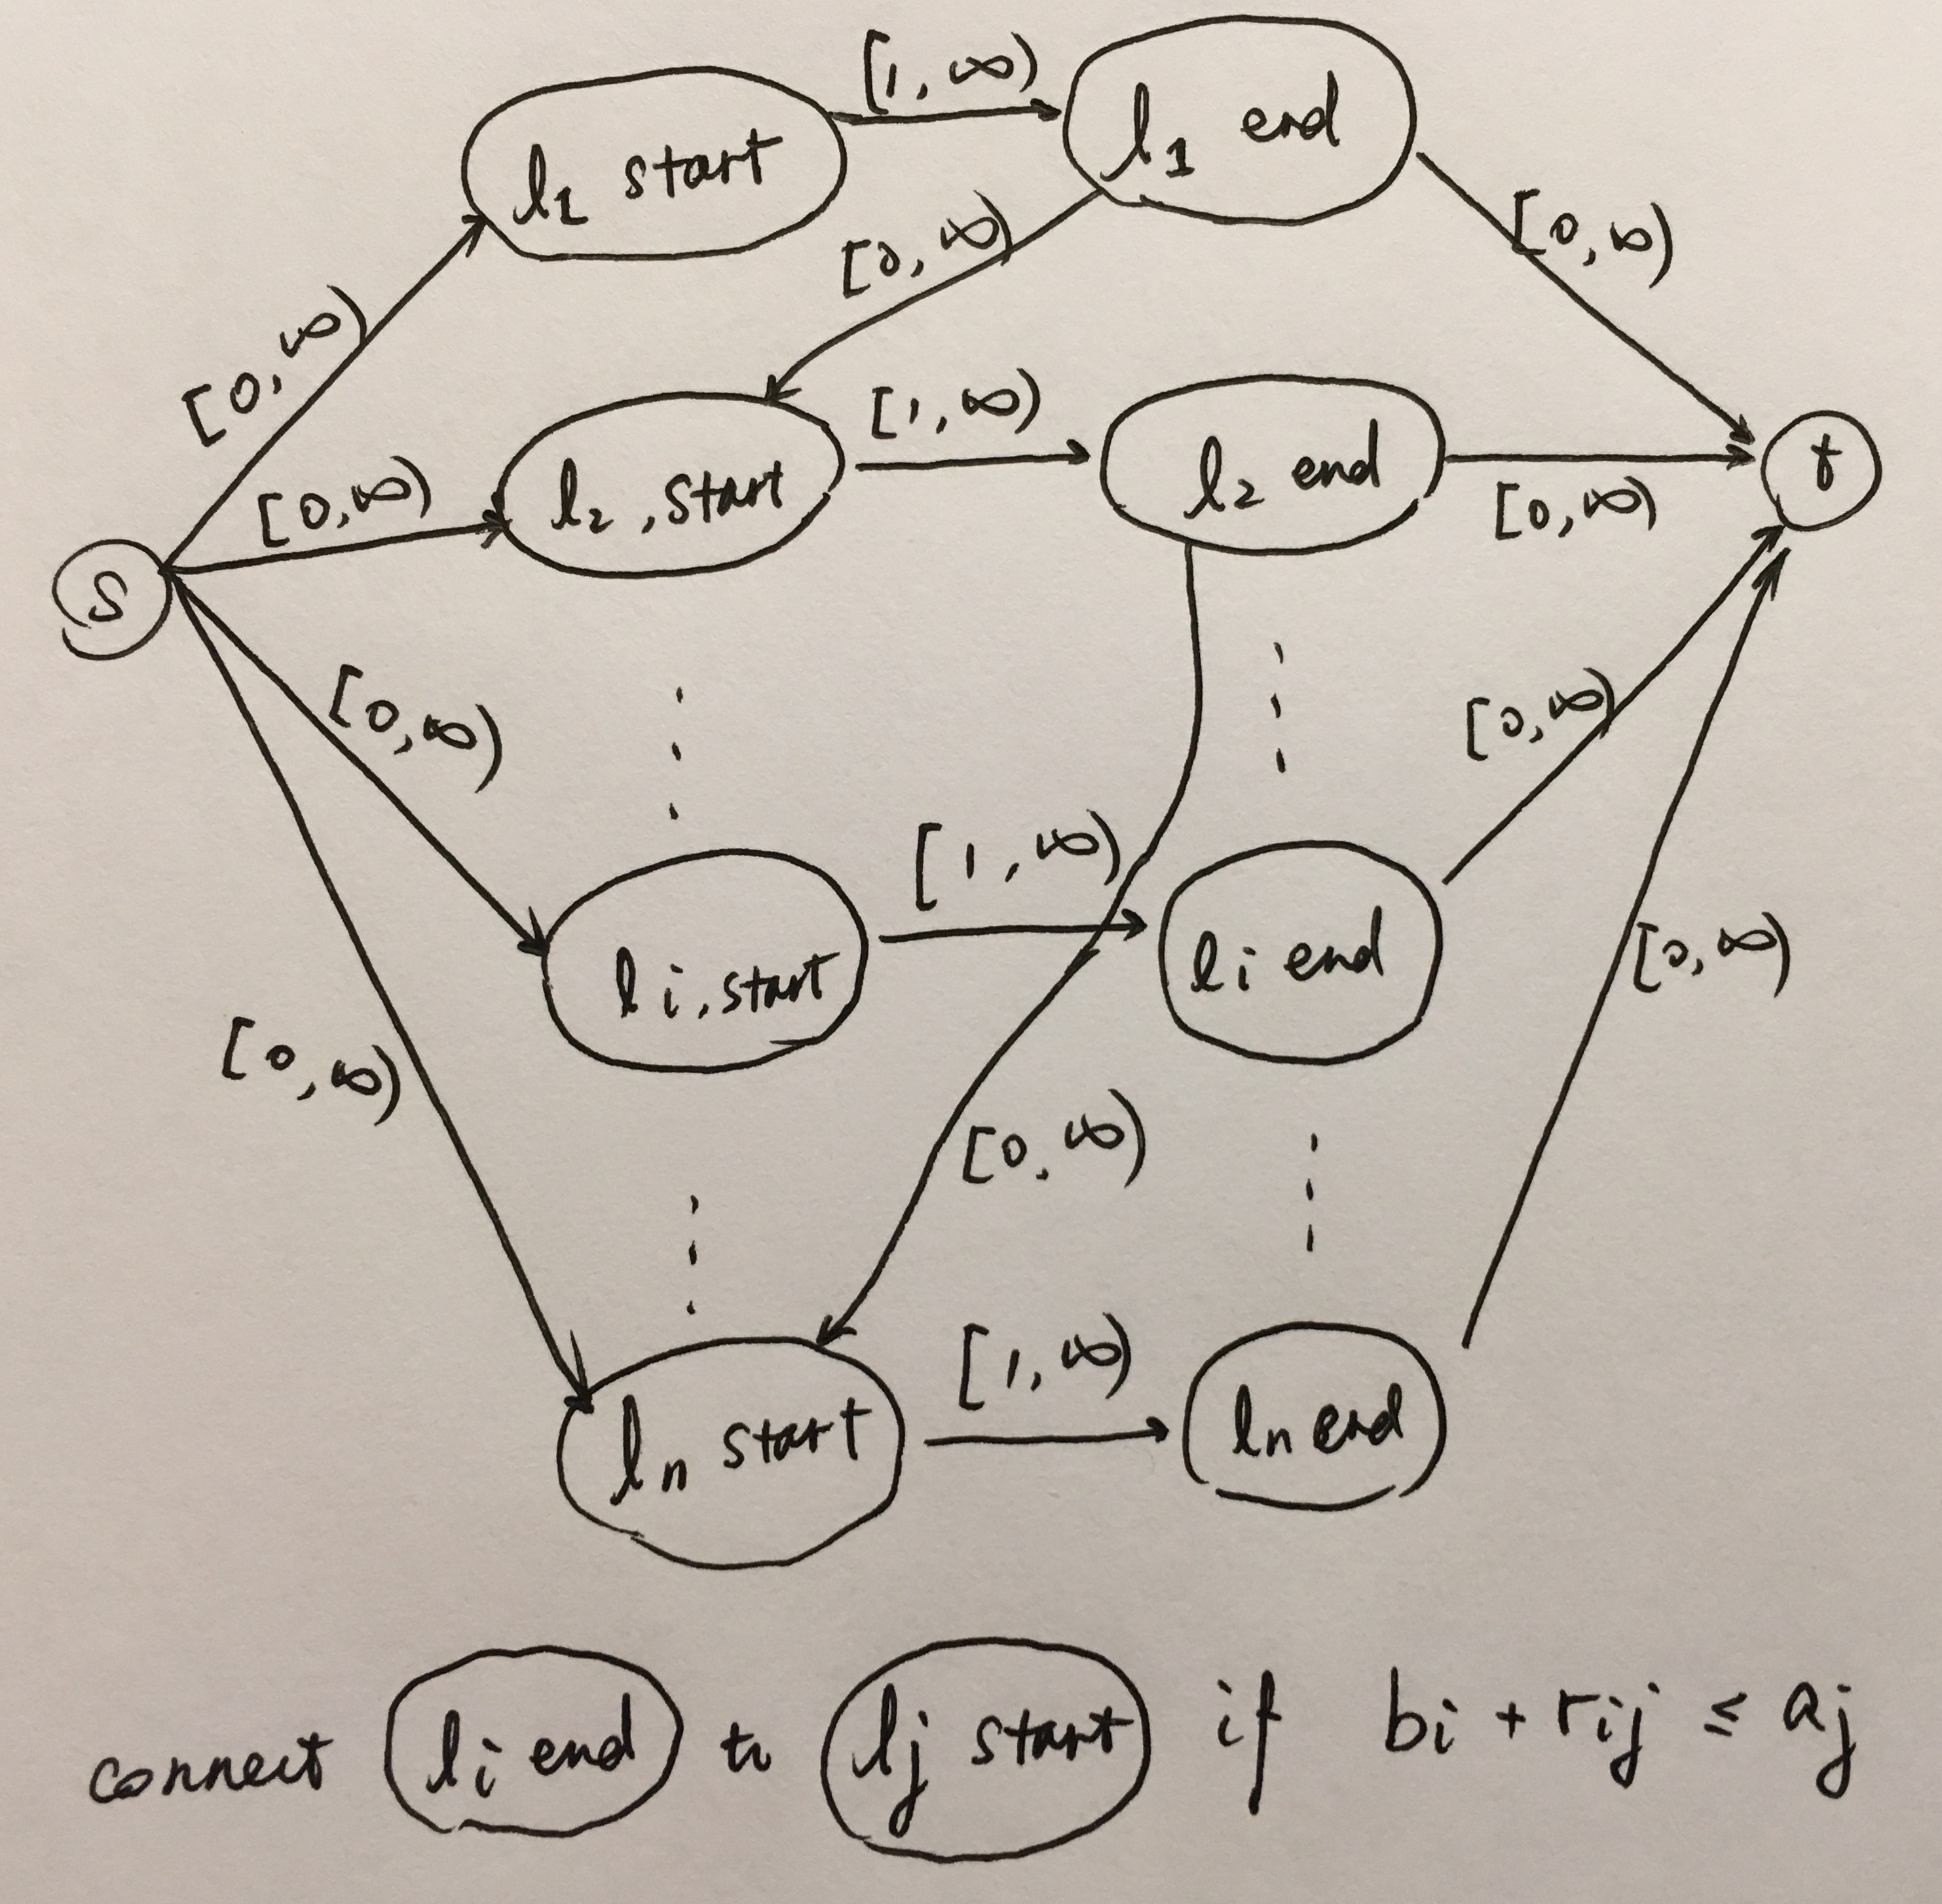
\includegraphics[width=0.6\textwidth]{2-c.jpg}
	\caption{Illustration of graph for minimum lecture attendance problem. Each edge has capacity constrained denoted as $[lower\_bound, upper\_bound]$. In this example, $b_1 + r_{12} \leq a_2$ and $b_2 + r_{2n} \leq a_n$.} \label{fig:2-c}
\end{figure}

Therefore, we dedicate a \emph{start} and a \emph{end} node for each lecture $i$, and connect an edge with capacity constraint $[1, +\infty)$ between them. This means each lecture should have at least one student flow through, checking the attendance. Then for every $i$ and $j$ satisfying $b_i + r_{ij} \leq a_j$, we connect an edge between node $l_{i,end}$ to $l_{j,start}$, indicating a student can go to lecture $j$ after attending lecture $i$. The capacity of this edge is unconstrained (set to $[0, +\infty)$). Next, connect source $s$ to every $l_{i,start}$ node with unconstrained edge and connect every $l_{i,end}$ node to sink $t$ also with unconstrained edge. An illustration is shown in Figure \ref{fig:2-c}. Finally, running a minimum flow over the graph constructed above will return a flow value indicating the minimum number of student required to attend all lectures.
 \pagebreak
  
\section*{Problem 3}
\paragraph{(a)} Recall that in the lecture we showed Dial's algorithm has running time $O(m+nC)$, where $nC$ is obtained because of $n$ \emph{delete-min}\footnote{Note that \emph{insert} and \emph{decrease-key} costs $O(1)$ time.} and operations and because each operation of finding the next min bounded by $O(C)$. Now, we instead analyze the running time for this entire operation. Notice that finding next checks the distance of nodes in a \emph{non-decreasing} fashion, as it scans \emph{forward} to find the next \emph{non-empty} bucket. Notice that the non-decreasing property holds even if some edges have 0 length. The buckets on the array therefore can be searched only once, which gives the total operation time $O(D)$ instead of $O(nC)$. Therefore, the total running time is $O(m+D)$, counting in traversing and checking every edge $m$ as before.  

\paragraph{(b)} Prove by contradiction. Suppose exists some $l_{vw}^d < 0$, thus $l_{vw} + d_v < d_w$. This means that the shortest path to $v$ plus the edge length from $v$ to $w$ is strictly smaller than the \emph{shortest} path to $w$, thus the new path via $v$ could have been the shortest path for $w$, which causes a contradiction. $\square$

\paragraph{(c)} We show (1) shortest paths on the original graph are the shortest paths on the reduced length graph and (2) shortest paths on the reduced length graph are the shortest paths on the original graph. 

(1) Consider a shortest path on the original graph, which has length $d_t$, where $t$ is the destination; the length on the reduced length graph would be 
$$l_{s,a_1}^d + l_{a_1,a_2}^d + \cdots + l_{a_n, t}^d = l_{s,a_1} + l_{a_1,a_2} + \cdots + l_{a_n, t} - d_t = 0.$$ Additionally, from (a) we know the reduced edge length has length $\geq 0$, therefore the shortest path on reduced graph is lower bounded by $0$. Therefore every shortest path on the original graph is a shortest path on the reduced length graph. 

(2) From (1) we know the shortest path on reduced length graph must have length 0. Then we immediately reach the same equation as above $0 = l_{s,a_1}^d + l_{a_1,a_2}^d + \cdots + l_{a_n, t}^d = l_{s,a_1} + l_{a_1,a_2} + \cdots + l_{a_n, t} - d_t.$ Therefore the same path has length equals to $d_t$ on the original graph, which indicates a shortest path. Thus all shortest paths on the reduced length graph are also shortest paths on the original graph. $\square$

The length of shortest paths on $l^d$ is 0, as shown in (1) above.

\paragraph{(d)} The scaling is on the bit level of original edge length $l$. First we express $l_{vw}$ in the binary form, then denote $l_{vw}^i$ as taking $i$ most significant bits\footnote{For example, taking 2 most significant bits of $(101)_2= 6_{10}$ is $(10)_2 = 3_{10}$.} of $l_{vw}$. Then we denote $d_v^i$ as shortest distance to node $v$ when lengths on the graph are $l_{vw}^i$. 

\subparagraph{Algorithm}
After solving a base problem on $l_{vw}^i$, the scaling step happens as follows. Let 
\begin{align*}
^d l^{i+1}_{vw} &= l^{i+1}_{vw} + 2d^i_v - 2d^i_w \\
&=2(l^{i}_{vw} + d^i_v - d^i_w) + \delta,
\end{align*}
where $\delta$ is either $0$ or $1$, depending on whether the shifting results in $l^{i+1}_{vw} = 2l^{i}_{vw} + 1$ or $l^{i+1}_{vw} = 2l^{i}_{vw}$, namely the new included bit is $0$ or $1$.

Now we run Dial's algorithm on the graph with $^d l^{i+1}_{vw}$ as the edge lengths. Notice that the path from $s$ to $t$ on this graph yields 
\begin{align*}
^d l_{s,a_1}^{i+1} + ^d l_{a_1,a_2}^{i+1} + \cdots + ^dl_{a_n, t}^{i+1} &= l_{s,a_1}^{i+1} + 2d^i_s - 2d^i_{a_1} + l_{a_1,a_2}^{i+1} + 2d^i_{a_1} - 2d^i_{a_2} + \cdots + l_{a_n, t}^{i+1} + 2d^i_{a_n} - 2d^i_t\\
&= l_{s,a_1}^{i+1} + l_{a_1,a_2}^{i+1} + \cdots + l_{a_n, t}^{i+1} - 2d^i_t
\end{align*}
Thus, the shortest distance obtained by Dial's algorithm, $^d d^{i+1}_t$ yields $^d d^{i+1}_t = d^{i+1}_t - 2d^i_t$. Because in the above, shortest distance is the min of the LHS of the equation, which must be also the minimum of RHS of the equation. As a result, we have the scaling relation, i.e. the shortest distance with $l_{vw}^i$ as edge lengths can be computed by $d^{i+1}_t = \:^dd^{i+1}_t + 2d^i_t$.

\subparagraph{Analysis} Each scaling step gives us shortest distance for the graph with $l_{vw}^i$ as edge lengths. The scaling is invoked $O(log\:n)$ times, as there is $O(log\:C)$ bits in edge length. In each scaling, notice that $^d l^{i+1}_{vw} =2(l^{i}_{vw} + d^i_v - d^i_w) + \delta$, from (a) we know Dial's algorithm is bounded by $O(m + D)$, where $D$ here has $D = 2(d^i_t - d^i_t) + \delta_1 + \delta_2 + ... + \delta_n \leq n\times \text{max}(\delta) = O(n)$. Therefore each Dial's algorithm is bounded by $O(m)$. In total, the algorithm costs $O(m\:log\:C)$.

\paragraph{(e)} In the scaling step, base-2 gives $^d l^{i+1}_{vw} = l^{i+1}_{vw} + 2d^i_v - 2d^i_w$, and similarly base-$k$ gives $^d l^{i+1}_{vw} = l^{i+1}_{vw} + kd^i_v - kd^i_w$, which at the end results in $O(kn)$ in each Dial's algorithm, and total scaling time $O(log_k\:C)$. Therefore, the algorithm running time is $O((m+kn)log_k\:C)$. Now take the derivative w.r.t. $k$, gives us $-\frac{(m+kn)log(C)}{k\:log(k)^2} + \frac{n\:log(C)}{log(k)}$. Letting this quantity equals zero gives us the optimal\footnote{Calculated by Mathematica. 

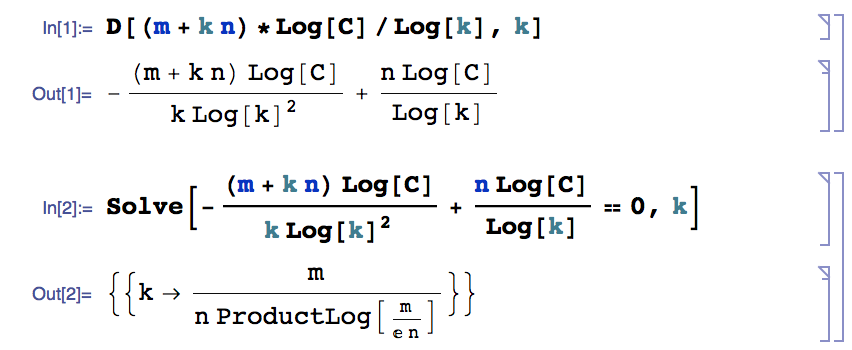
\includegraphics[width=0.4\textwidth]{3-e.png} \label{fig:3-e}

The trick for avoiding derivatives in Karger's lecture seem not to be working here: $m\:log_k\:C = kn\:log_k\:C$, not sure this is about one growing and one decaying variable, more like a decaying but with different speed, w.r.t. $k$. Nonetheless, if it can still apply, it gives a `optimal' base $k = m/n$, and running time $O(m\:log_{m/n}\:C)$} $k=\frac{m}{n\:ProductLog(m/(en))}$, where $ProductLog(\cdot)$ is the solution of $\cdot = xe^x$.
\pagebreak

\section*{Problem 4} 
\paragraph{(a)} In the admissible graph, there are $d + 1$ layers (counting source and sink individually) of vertices. Denote the number of vertices on layer $i$ to be $L_i$. Then we know $\sum_{i=1}^{d+1} L_i \leq n$. Consider \emph{adjacent} layers, we have $\sum_{i=1}^{d} (L_i + L_{i+1}) \leq 2n$. For these $d$ adjacent layers, we know $\text{max}\big\{\text{min}_i\{L_i + L_{i+1}\}\big\} \leq 2n/d$, this is because at this value any increasing of number of vertices in a layer pair reduces the vertices on some other layer pairs, resulting in a smaller min. Similarly, between two adjacent layers, the min value of the pair is $(2n/d)/2 = n/d$, for the same argument. Therefore, the value of maximum flow is upper bounded by $\left(n/d\right)^2$.

Now consider we operate $k$ blocking flows. This means, in the residual graph, the distance between $s$ and $t$ is at least $k$. Then, the max flow is upper bounded by $(n/k)^2$. With a max flow $(n/k)^2$, there is at most $(n/k)^2$ more blocking flows. Notice here $k$ can be arbitrary, therefore we set $k$ to minimize $k+(n/k)^2$. Let\footnote{The trick for avoiding derivatives in Karger's lecture.} $k=(n/k)^2$, we obtain $k=n^{2/3}$ and total number of blocking flow can be bounded by $O(n^{2/3})$. 
\paragraph{(b)} From part (a) we know the distance between source and sink is bounded by $n / \sqrt{f}$. Now we consider the length of shortest augmenting paths that were used to reach flow $f$. Notice the intuition that if the distance between source and sink is small, then the length of the path would be small, since we choose the shortest path when augmenting the flows. The number of edges can be upper bounded by the sum of the lengths of the flow paths. The length of the flow is bounded by the distance $n / \sqrt{f}$. Therefore, we know the total number of edges can be bounded by $O(n/\sqrt{f} \times f) = O(n \sqrt{f})$.
\pagebreak

\section*{Problem 5}
\paragraph{(a)} Notice first that the directed graph needs to be strongly connected for every node, i.e. every node can be reached from any other node, in order for the street sweeping problem to have a solution. This is because the source node must be able to reach any node and any node must have path to the source node, otherwise the street-cleaner would be `trapped'. Via source node, any node can be reached from any other node.

If a directed graph is \emph{Eulerian}, the street sweeping problem has optimal total distance equals to sum of all edge distance, because of the well-known theorem. When the directed graph is \emph{non-Eulerian}, e.g. Figure \ref{fig:5-a}, it means some vertices have more outgoing edges than incoming edges, and some vertices have more incoming edges than outgoing edges. For those vertices with more incoming edges, e.g. $A$ in Figure \ref{fig:5-a}, \emph{some} outgoing edges have to be used multiple times; and similarly but reverse situation applies to nodes with more outgoing edges, e.g. $D$ in Figure \ref{fig:5-a}.
\begin{figure}[h!]
	\centering
	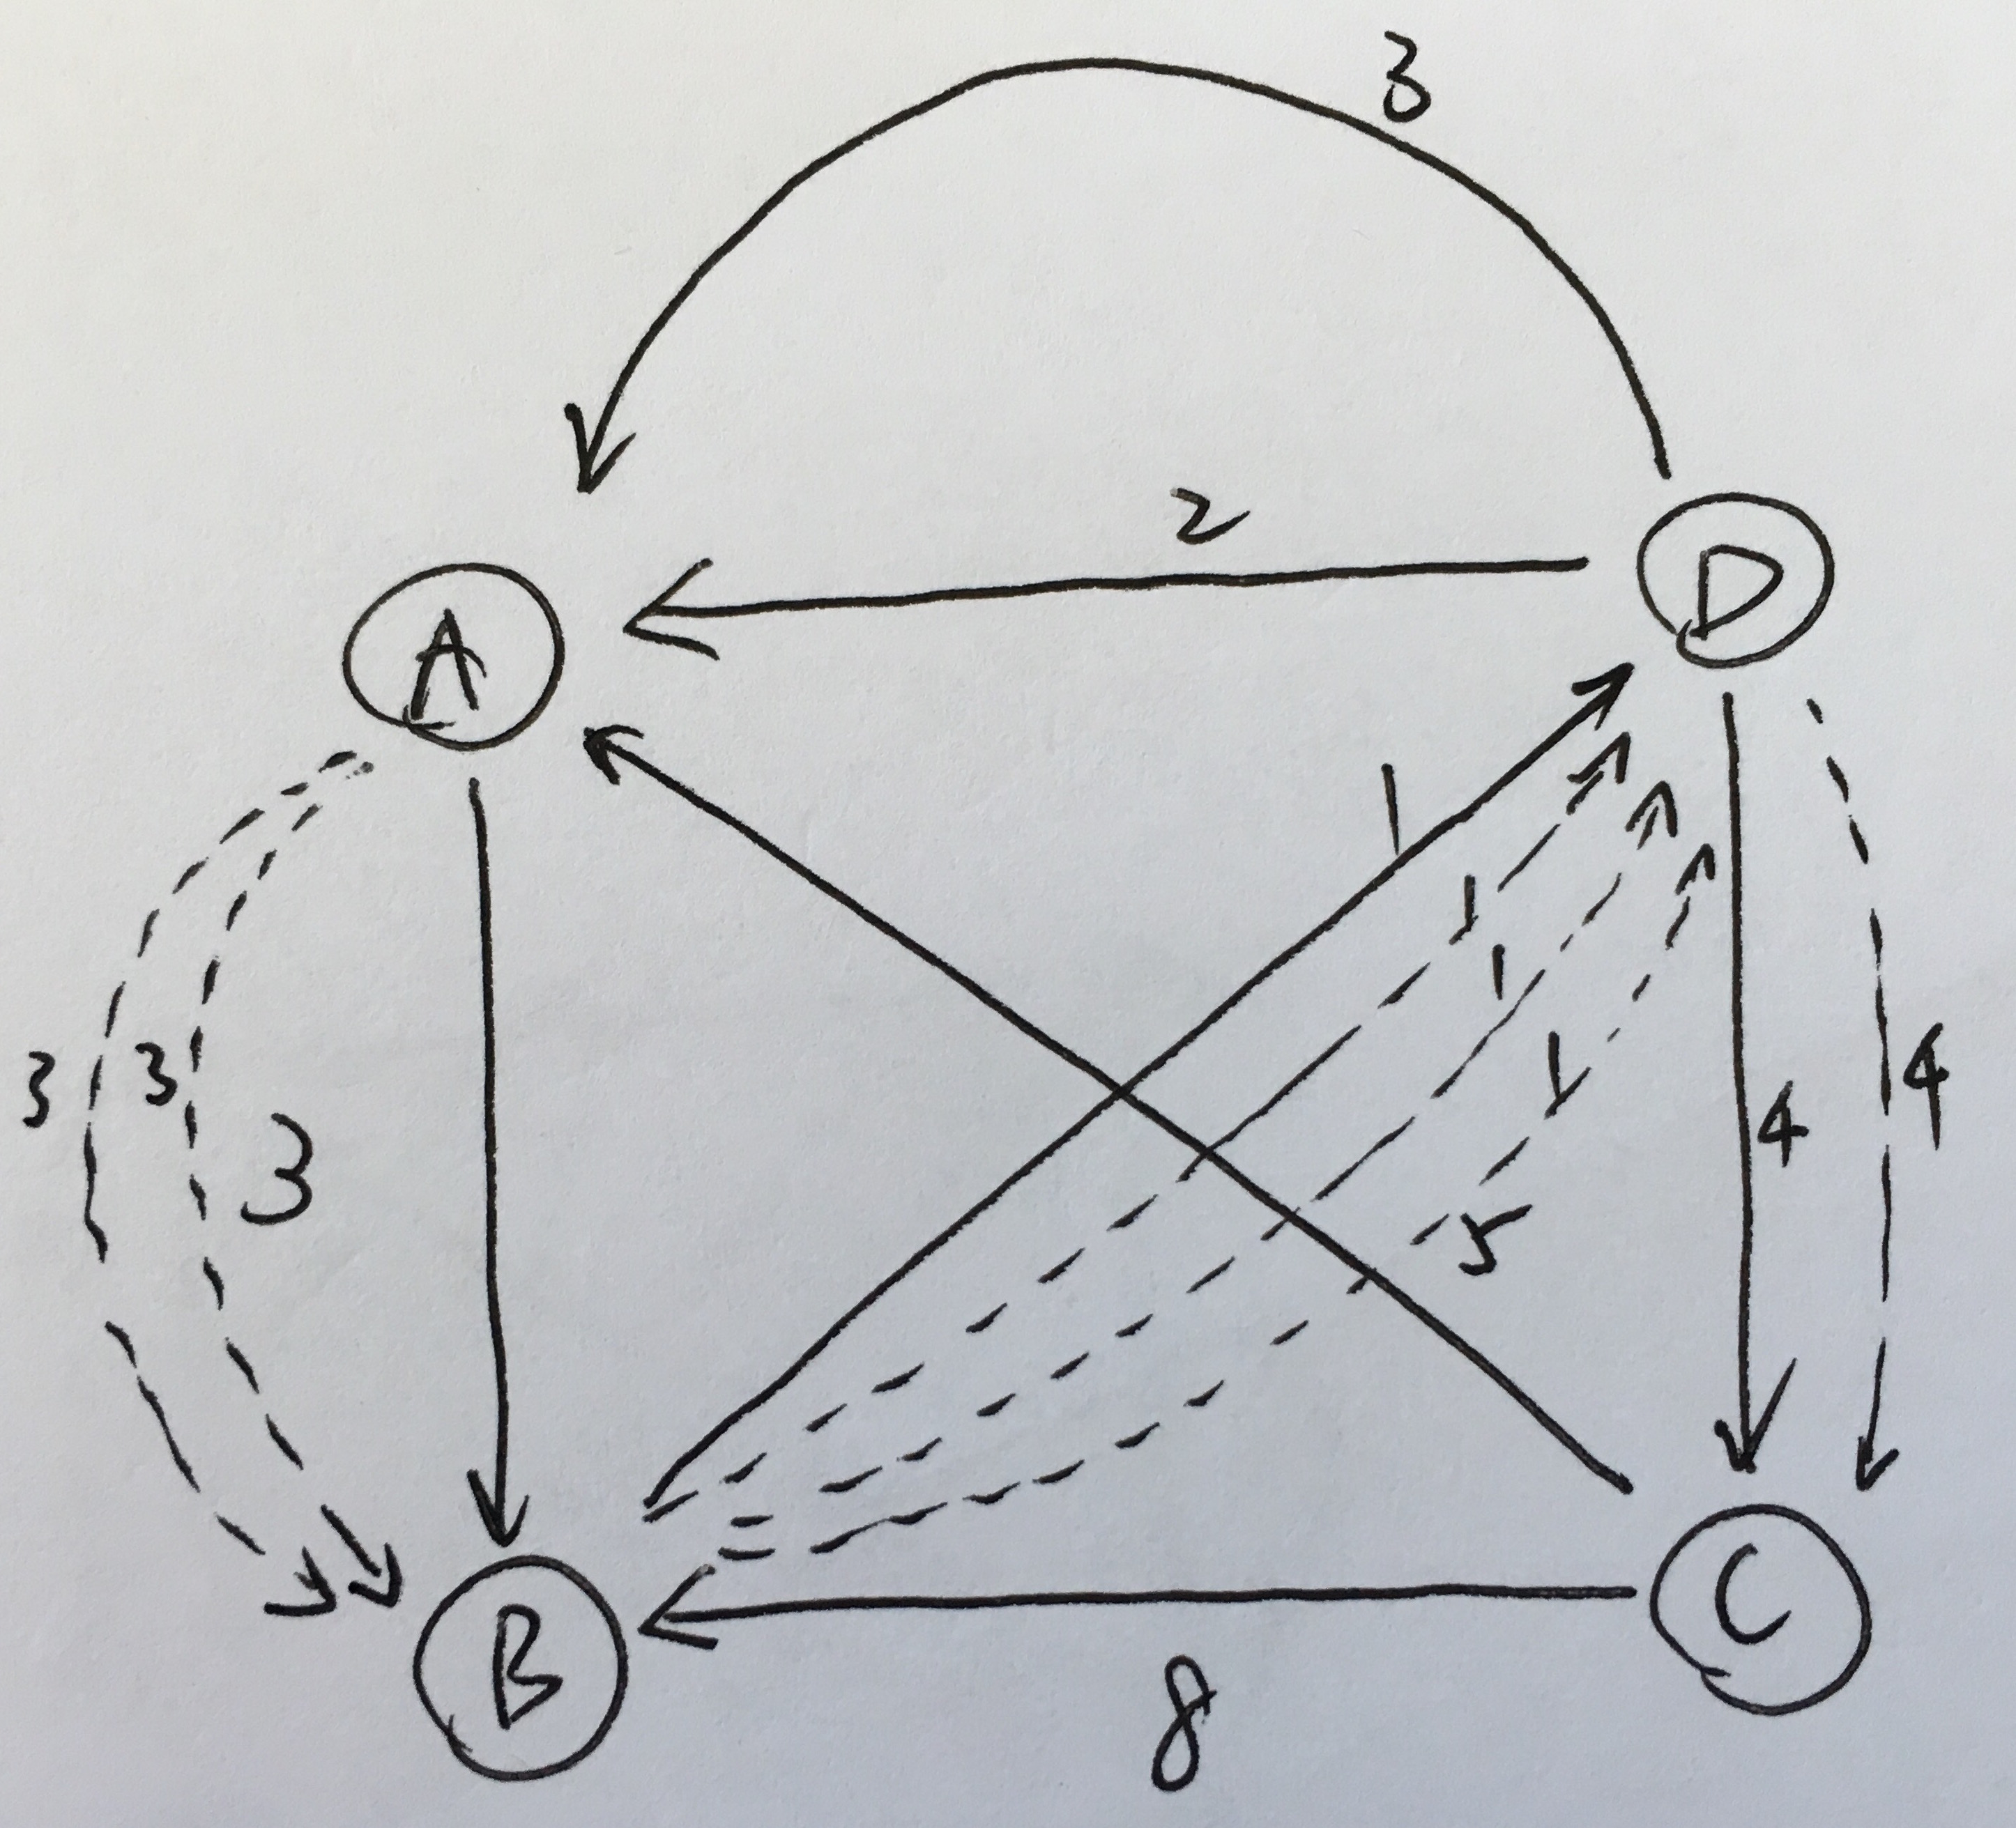
\includegraphics[width=0.4\textwidth]{5-a.jpg}
	\caption{An example of non-Eulerian directed graph. The number on edges denote the cost of edge traversal. Dashed arrows indicate the edges that need to be traversed multiple times. The additional fictitious edges make the graph Eulerian.} \label{fig:5-a}
\end{figure}

In the optimal solution, we know some those edges are traversed multiple time. Now we assume first in this ub-problem that we have those ``minimum cost'' set of edges in hand, and we will solve in (b) how to use min-cost flow to find them. Then, we can copy those edges into the graph to make the graph Eulerian. Specifically, an edge is copied $n$ times if it is traversed $n+1$ times in the optimal street sweeping route. For example, in \ref{fig:5-a}, edge $e(A,B)$ and $e(B,S)$ is traversed \emph{twice} and those edges are copied into the graph. The new graph becomes Eulerian because the number of incoming edges are equal to the number of outgoing edges for all vertices, as all edges need to be traversed exactly once. Now the sum of all edge distances in this new Eulerian graph is the optimal total distance the street cleaner needs to travel.

\subparagraph{(b)} For a vertex that has $k$ more incoming edges than outgoing edges, it needs to use a set of some of its outgoing edges $k$ more times for optimal total distance. If it is less than $k$ than some incoming edges can not be covered. \emph{Only consider this vertex}\footnote{Others can use a edge multiple times for covering their edges, e.g. in Figure \ref{fig:5-a}, but the argument here focuses on the current vertex alone.}, if it is more than $k$ then some incoming edges are covered more than once, which is suboptimal. Similar case applies to vertices with more outgoing edges than incoming edges.
\begin{figure}[h!]
	\centering
	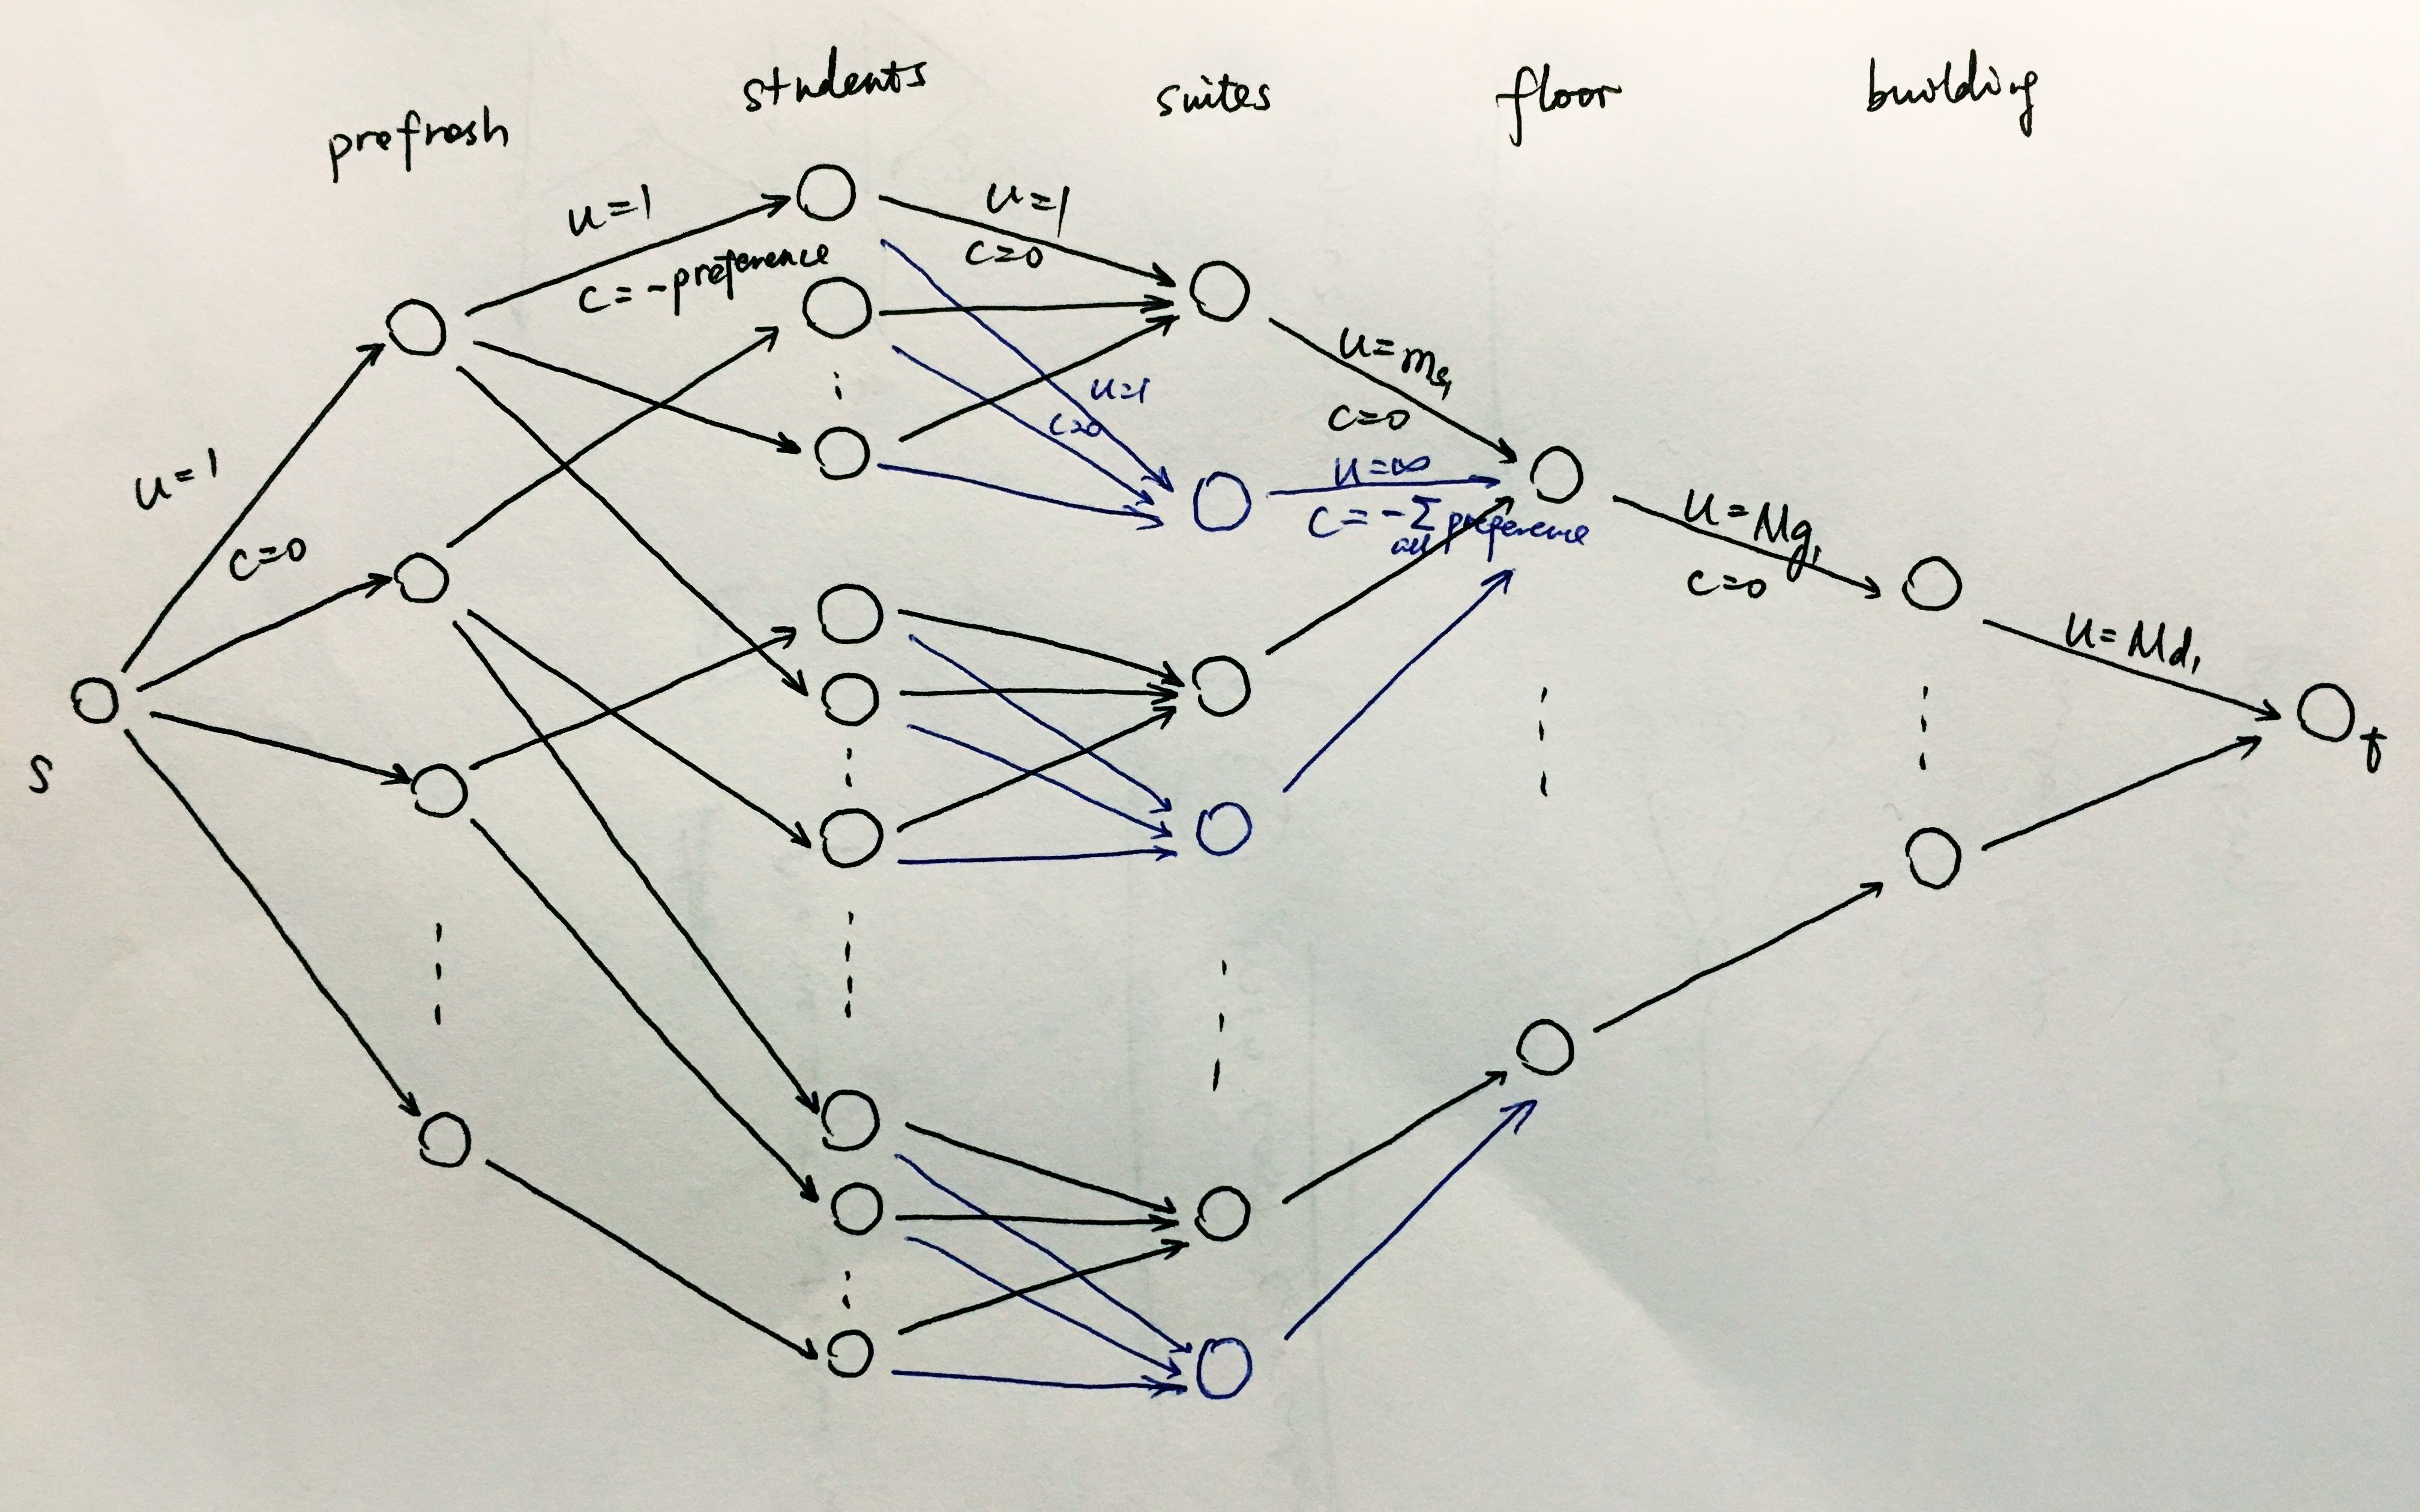
\includegraphics[width=1\textwidth]{5-b.jpg}
	\caption{Finding minimum cost set of edges to add using min cost flow. The ``more incoming'' group has node $A$ $B$ and super source $S^*$ and the ``more outgoing'' group has node $C$ $D$ and super sink $T^*$. On the link $r=\cdot$, denotes the required flow amount, $c=\cdot$ denotes the flow cost. Links without $r$ have no constraint on the capacity. Colored flow indicate \emph{a} min-cost flow ($1+4+8 = 13 \leq 5 + 4 \times 2$), which translates to the dashed edges added on the left figure.} \label{fig:5-b}
\end{figure}

Therefore, we can construct another graph separating all vertices with more incoming edges and vertices with more outgoing edges. An example is shown in Figure \ref{fig:5-b}. In Eulerian graph, the total number of incoming edges matches with total number of outgoing edges. Thus, we can pair the vertices in these two groups. More specifically, for a vertex with $k$ more incoming edges, we connect it to a source node, with edge requirement $r=k$ and cost $c=0$; and for a vertex with $k$ more outgoing edges, we connect it to a sink node, with edge requirement $r=k$ and cost $c=0$. For any two nodes across two groups, we first run a shortest path algorithm on the \emph{original} graph and obtain the minimum distance $d$, then we connect the pair with an edge of $c=d$. Then, we run min-cost flow on the newly constructed graph from source to sink. Notice that the resulting min-cost flow represent the total minimum distance of edges to be added. Next, for each edge connecting two pairs, that has flow through, we add corresponding amount of edges on the original graph, along the shortest path connecting the two vertices. Finally, we reach the state of (a) and we can use Eulerian graph to solve the street sweeping problem.

\end{document}